\documentclass{beamer}
\usepackage{pgfpages}
\usepackage[backend=bibtex]{biblatex}
\usepackage{multicol}
\usepackage{multimedia}
\usepackage[absolute,overlay]{textpos}
\usepackage{parskip}
\usepackage{hyperref}
\usepackage{lmodern}
\usepackage{bbding}
\usepackage[absolute,overlay]{textpos}
\usepackage{framed} %Used to shade important equations, color devined with shadecolor
\usepackage{url}
\hypersetup{colorlinks=true, urlcolor=blue}
\setlength{\parskip}{\smallskipamount}
\colorlet{shadecolor}{cyan}
%\usepackage[texcoord,grid,gridunit=mm,gridcolor=red!10,subgridcolor=green!10]{eso-pic} %DELETE when done with grid
\setbeameroption{hide notes} % Only slides
%\setbeameroption{show only notes} % Only notes
%\setbeameroption{show notes on second screen=right} % Both
%\bibliography{../../papers/references.bib}
\setbeamerfont{footnote}{size=\tiny}
%\AtEveryCitekey{\clearfield{title}}

%
% Choose how your presentation looks.
%
% For more themes, color themes and font themes, see:
% http://deic.uab.es/~iblanes/beamer_gallery/index_by_theme.html
%
\mode<presentation>
{
\usetheme{Warsaw}      % or try Darmstadt, Madrid, Warsaw, ...
\usecolortheme{default} % or try albatross, beaver, crane, ...
\usefonttheme{default}  % or try serif, structurebold, ...
\setbeamertemplate{navigation symbols}{}
\setbeamertemplate{caption}[numbered]
} 

\usepackage[english]{babel}
%\usepackage[utf8x]{inputenc} %Doesn't play well with biblatex
\usepackage{amssymb}
\usepackage{bm}
\usepackage{color}
\usepackage{graphicx}
\setbeamercovered{invisible}
\setbeamercovered{%
again covered={\opaqueness<1->{100}}} %This changes the opaqueness of each bullet

\newcommand{\red}[1]{{\color{red}{#1}}}
\newcommand{\checkH}[2]{\begin{textblock*}{1cm}(#1,#2){\Huge \red{\Checkmark}}\end{textblock*}}
\newcommand{\checkh}[2]{\begin{textblock*}{1cm}(#1,#2){\huge \red{\Checkmark}}\end{textblock*}}
\newcommand{\checkL}[2]{\begin{textblock*}{1cm}(#1,#2){\Large \red{\Checkmark}}\end{textblock*}}
\newcommand{\checkl}[2]{\begin{textblock*}{1cm}(#1,#2){\large \red{\Checkmark}}\end{textblock*}}
\renewcommand{\rm}[1]{\mathrm{#1}}

\title[{\color{white}{Heat Transfer - Radiation}}]{Radiation as a Mechanism for Heat Transfer}
\author{Cody Petrie}
\institute{Southern Utah University}
\date{}

\begin{document}

%\setbeamertemplate{frametitle}[default][center]
\begin{frame}
\titlepage
\end{frame}

% Uncomment these lines for an automatically generated outline.
%\begin{frame}{Outline}
%  \tableofcontents
%\end{frame}

% Commands to include a figure:
%\begin{figure}
%\includegraphics[width=\textwidth]{your-figure's-file-name}
%\caption{\label{fig:your-figure}Caption goes here.}
%\end{figure}

\begin{frame}{Quiz}
\begin{center}
{\Large NO QUIZ TODAY}
\end{center}
I was told that that my lesson can't have any effect on your grades
\end{frame}

\begin{frame}[t]{Radiation}
What do you think of when you hear the word radiation?
\only<2->{
   \begin{textblock*}{\textwidth}(0.3cm,1.8cm) % {block width} (coords)
      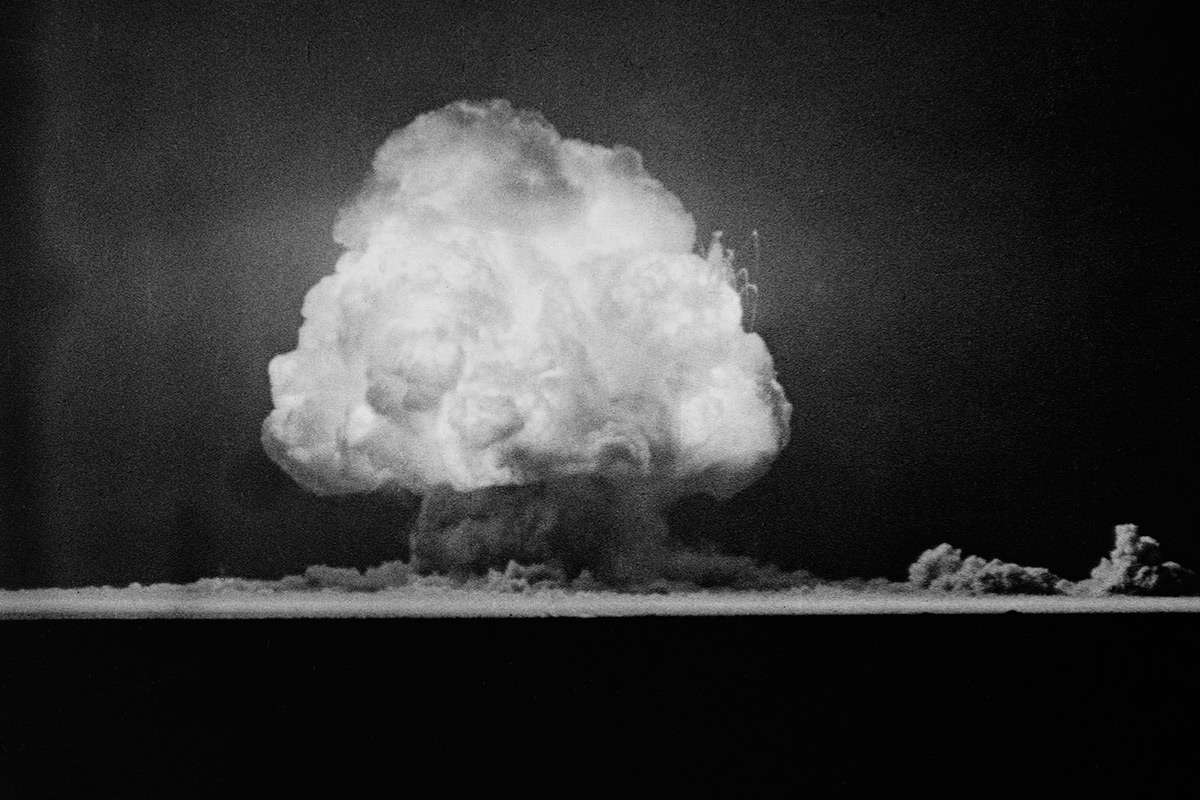
\includegraphics[width=8.0cm]{figures/trinity.jpg}
   \end{textblock*}
}
\only<3->{
   \begin{textblock*}{\textwidth}(7.5cm,2.0cm) % {block width} (coords)
      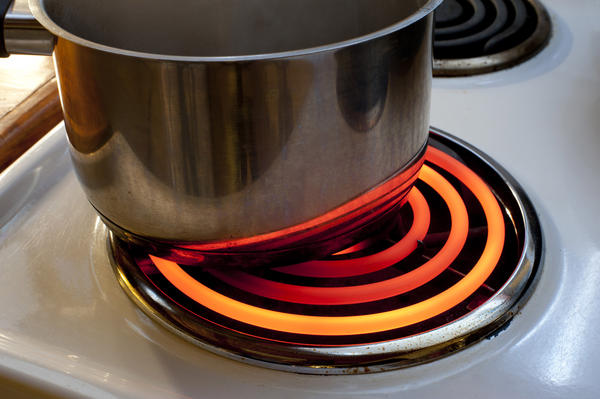
\includegraphics[width=4.5cm]{figures/pan_on_stove.jpg}
   \end{textblock*}
   \begin{textblock*}{\textwidth}(6.5cm,5.6cm) % {block width} (coords)
      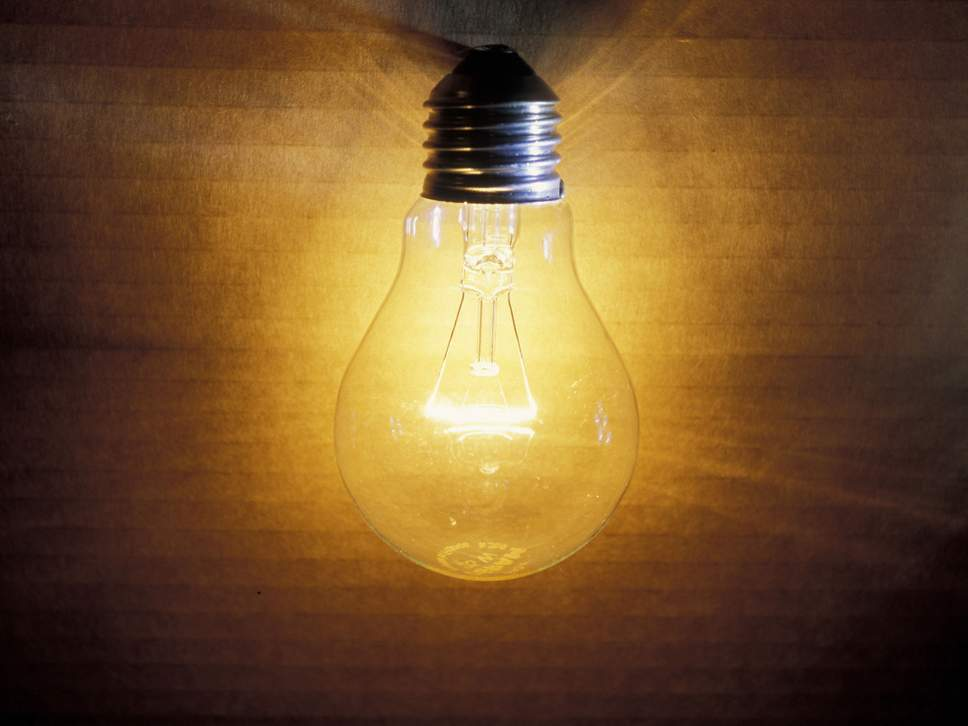
\includegraphics[width=4.5cm]{figures/light_bulb.jpg}
   \end{textblock*}
}
\only<4->{
   \begin{textblock*}{\textwidth}(2.5cm,3.0cm) % {block width} (coords)
      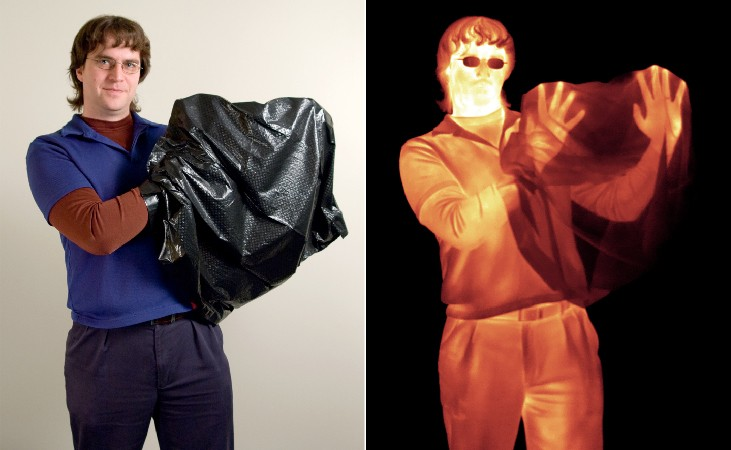
\includegraphics[height=5.0cm,trim={0 0 13cm 0},clip]{figures/infrared.jpg}
   \end{textblock*}
}
\only<5->{
   \begin{textblock*}{\textwidth}(2.5cm,3.0cm) % {block width} (coords)
      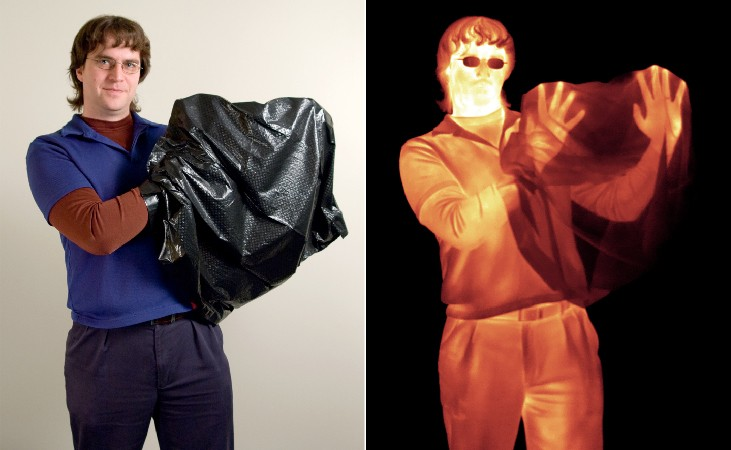
\includegraphics[height=5.0cm]{figures/infrared.jpg}
   \end{textblock*}
}
\only<6->{
   \begin{textblock*}{\textwidth}(2.0cm,2.3cm) % {block width} (coords)
      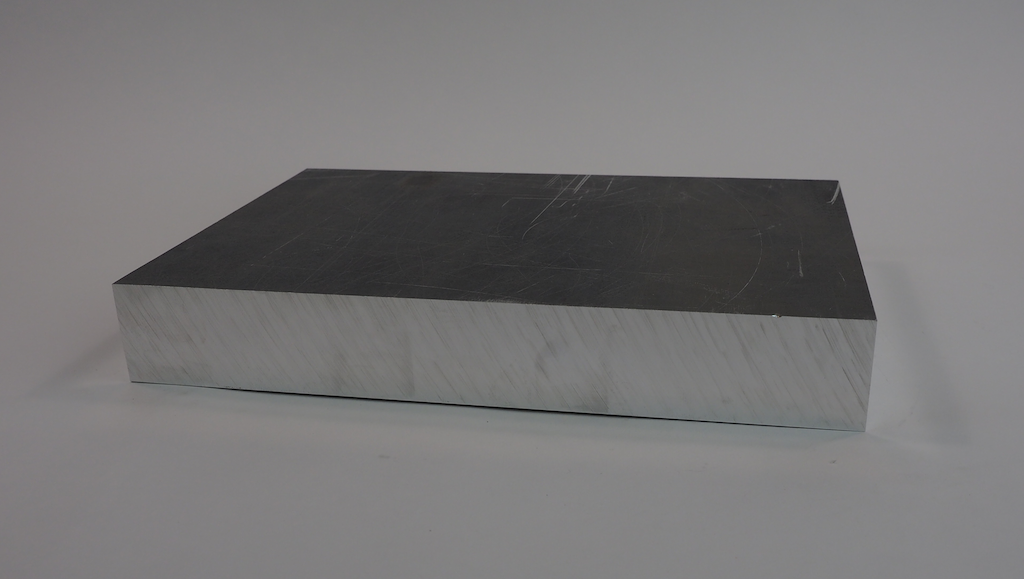
\includegraphics[width=10.0cm]{figures/metal.png}
   \end{textblock*}
}
\end{frame}

\begin{frame}[t]{Review}
\begin{itemize}
   \item Before we talk more about radiation let's all get on the same page.
   \item<2-> What is {\bf internal energy}?
   \begin{itemize}
      \item<3-> The energy of all of the internal pieces (atoms and molecules) of an object, as seen at rest.
   \end{itemize}
   \item<4-> What about {\bf work} and {\bf heat}?
   \begin{itemize}
      \item<5-> Work is energy being transfered by some force.
      \begin{align*}
         dW&=\mathbf{F}\cdot d\mathbf{r}~~~~~~~~~~~~~~~~~~~~~~~~~~~~~~~~\\
         dW&=-PdV~~~~~~~~~~~~~~~~~~~~~~~~~~~~~~~~
      \end{align*}
      \vspace{-0.8cm}
      \item<6-> Heat is the flow of energy from one thing to \\ another, usually because of a temperature \\ difference.
   \end{itemize}
\end{itemize}
\only<3->{
   \begin{textblock*}{\textwidth}(9.5cm,3.5cm) % {block width} (coords)
      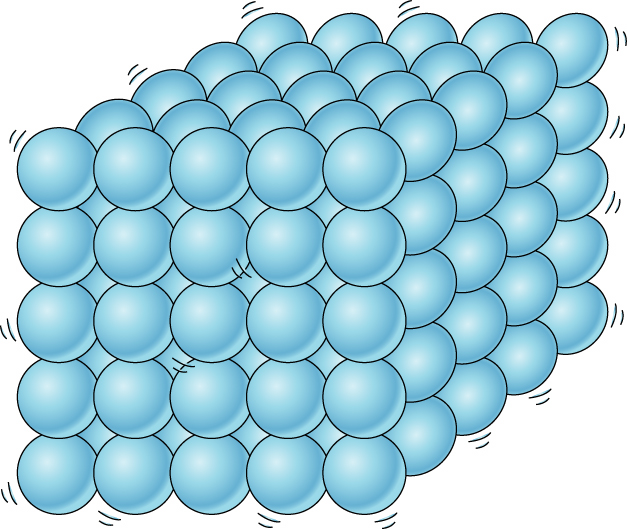
\includegraphics[width=3.0cm]{figures/vibrating_solid.jpg}
   \end{textblock*}
}
\only<5->{
   \begin{textblock*}{\textwidth}(1.0cm,7.3cm) % {block width} (coords)
      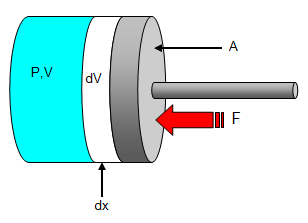
\includegraphics[width=3.0cm]{figures/work.png}
   \end{textblock*}
}
\only<6->{
   \begin{textblock*}{\textwidth}(4.0cm,6.9cm) % {block width} (coords)
      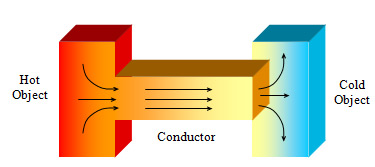
\includegraphics[width=5.0cm]{figures/heat_flow.jpg}
   \end{textblock*}
}
\end{frame}

\begin{frame}[t]{First Law of Thermodynamics}
\begin{itemize}
   \item With these three things ($E_\text{int}$, $W$, $Q$) can you remember what the first law of thermodynamics is {\bf and what it means}?
   \only<2->{
   \begin{equation*}
      \Delta E_\text{int} = Q + W
   \end{equation*}
   }
   \item<3-> Are those heat {\bf taken from} or {\bf added to}, and work {\bf done on} or {\bf done by} the system? {\it Discuss with the person next to you until you agree on something.}
   \only<4->{
   \begin{equation*}
      \Delta E_\text{int} = Q_\text{added to} + W_\text{done on}
   \end{equation*}
   }
\end{itemize}
\end{frame}

\begin{frame}[t]{Check for Understanding}
\begin{center}
   I have a gas contained in a metal cylinder with a piston. I want to temporarily raise the energy of the gas contained in a cylinder. How should I do it and how much will it change the energy by?
   \begin{textblock*}{\textwidth}(5.0cm,3.0cm) % {block width} (coords)
      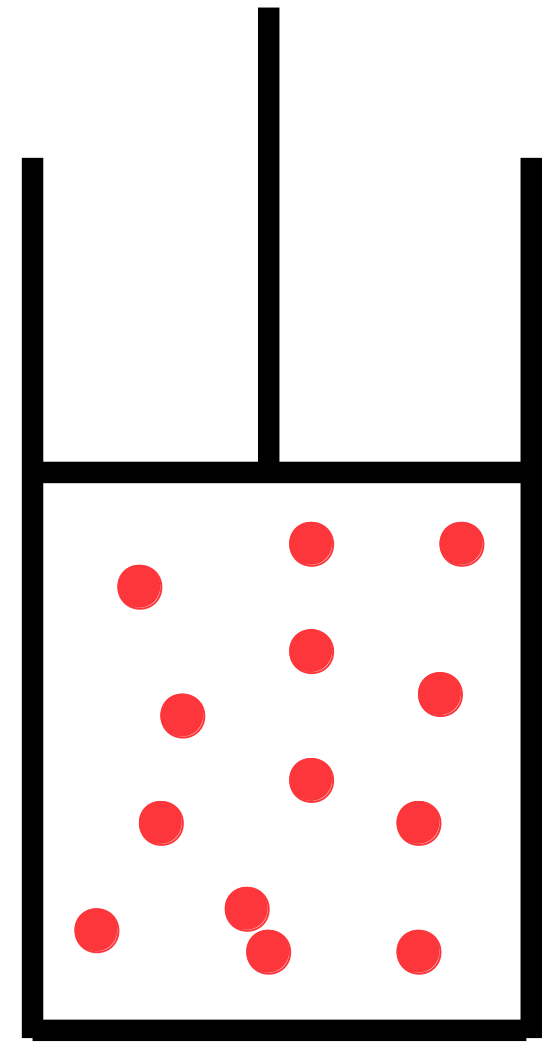
\includegraphics[width=3.0cm]{figures/mypiston.png}
   \end{textblock*}
   \begin{enumerate}[A.]
      \item Push the piston down, $\Delta E\text{int} = \int\limits_{V_i}^{V_f} PdV$
      \item Push the piston down, $\Delta E\text{int} = -\int\limits_{V_i}^{V_f} PdV$
      \item Pull the piston up, $\Delta E\text{int} = \int\limits_{V_i}^{V_f} PdV$
      \item Pull the piston up, $\Delta E\text{int} = -\int\limits_{V_i}^{V_f} PdV$
      \item Quit and give up
   \end{enumerate}
\only<2>{\checkl{0.5cm}{4.0cm}}
\end{center}
\end{frame}

\begin{frame}[t]{Check for Understanding - Again}
\begin{center}
   Same situation, we want to add energy, but since we used a metal cylinder the piston rusted over. What should we do now to add energy?
   \begin{textblock*}{\textwidth}(5.0cm,3.0cm) % {block width} (coords)
      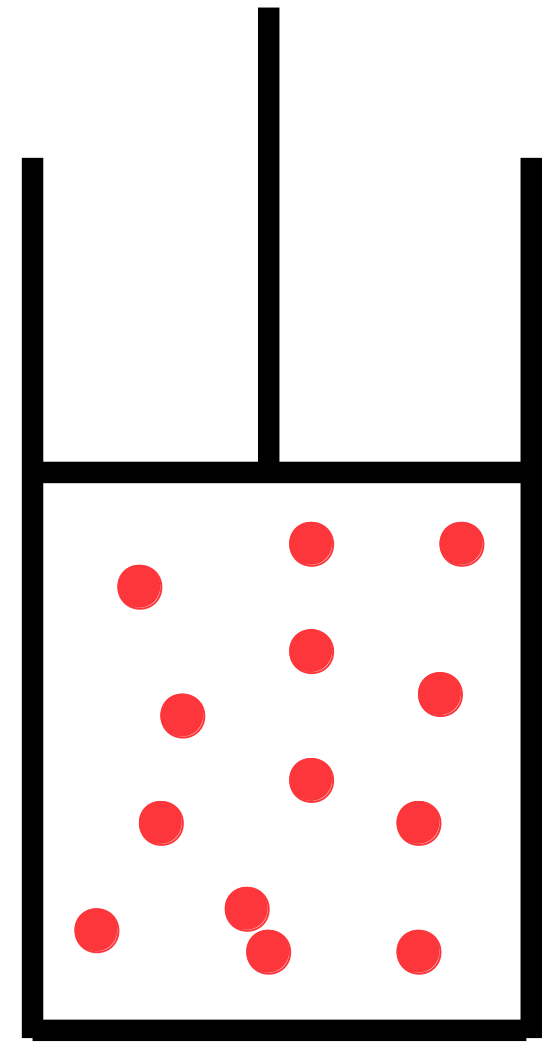
\includegraphics[width=3.0cm]{figures/mypiston.png}
   \end{textblock*}
   \begin{enumerate}[A.]
      \item Keep pushing on the piston
      \item Wait for a really long time for something to \\ happen
      \item Give up, but give the container a good hard \\ kick to make us feel better
   \end{enumerate}
\only<2>{\checkl{0.5cm}{4.1cm}}
\end{center}
\only<2>{\Large ~\\~\\And this leads us into our \\ next topic: heat transfer
}
\end{frame}

\begin{frame}{Picture References}
\tiny
Trinity bomb, accessed 28 Feb 2019: \href{https://www.newscientist.com/article/2120748-glass-from-nuclear-test-site-shows-the-moon-was-born-dry/}{https://www.newscientist.com/article/2120748-glass-from-nuclear-test-site-shows-the-moon-was-born-dry/}\\
Pan on stove, accessed 28 Feb 2019: \href{https://stockarch.com/images/business-and-industry/energy/pan-red-hot-hotplate-8009}{https://stockarch.com/images/business-and-industry/energy/pan-red-hot-hotplate-8009}\\
Light bulb, accessed 28 Feb 2019: \href{https://www.independent.co.uk/news/science/old-fashioned-light-bulbs-could-be-set-for-comeback-after-light-recycling-breakthrough-a6806446.html}{https://www.independent.co.uk/news/science/old-fashioned-light-bulbs-could-be-set-for-comeback-after-light-recycling-breakthrough-a6806446.html}\\
Infrared man, accessed 28 Feb 2019: \href{https://courses.lumenlearning.com/astronomy/chapter/visible-light-detectors-and-instruments/}{https://courses.lumenlearning.com/astronomy/chapter/visible-light-detectors-and-instruments/}\\
Block of metal, accessed 28 Feb 2019: \href{http://beatty-robotics.com/metalbot-work-in-process/}{http://beatty-robotics.com/metalbot-work-in-process/}\\
Vibrating solid, accessed 28 Feb 2019: \href{https://chemstuff.files.wordpress.com/2012/06/image137.jpg}{https://chemstuff.files.wordpress.com/2012/06/image137.jpg}\\
Piston, accessed 28 Feb 2019: \href{http://www.schoolphysics.co.uk/age16-19/Thermal\%20physics/Thermodynamics/text/Work_done_by_an_ideal_gas/index.html}{http://www.schoolphysics.co.uk/age16-19/Thermal\%20physics/Thermodynamics/text/Work\_done\_by\_an\_ideal\_gas/index.html}\\
Heat flow, accessed 28 Feb 2019: \href{http://www.ecd.com/support/learning-center/resources/heat-flow-happens.aspx?Post=3899\&tabid=371}{http://www.ecd.com/support/learning-center/resources/heat-flow-happens.aspx?Post=3899\&tabid=371}
\end{frame}

\end{document}
